\documentclass{beamer}
\usecolortheme{wolverine}

\usepackage[utf8]{inputenc}

\usepackage{graphicx}
\usebackgroundtemplate%
{%
    
\includegraphics[width=\paperwidth]{Images/fondoflisol.png}%
}


\title{Sofware Libre, más allá de lo evidente}
\author{Víctor Orozco}
\institute{Shekalug}
\date{26/04/2014}

\begin{document}

\frame{\titlepage}

\section{Intro}

\begin{frame}{Yo}
    \begin{itemize}
    \item Ing. Msc.
    \item Oracle, Java
    \item Tiempo libre: Shekalug, Guatejug, Gentoo
    \item Arquitecto JEE
    \item Becario OEA-GCUB - GtSeg
    \item Verdadero tiempo libre: Café, idiomas, musica, correr
    \end{itemize}
\end{frame}

\begin{frame}
\frametitle{Software Libre}
    \begin{figure}[tbph]
        \centering
        
\includegraphics[width=0.5\linewidth]{Images/why.png}
        \label{fig:CyberCommand}
    \end{figure}
\end{frame}


\begin{frame}{Software Libre}
    \begin{itemize}
        \item El software siempre fue libre
        \item El software inicio a ser negocio
        \item Xerox vs. RMS
        \item Proyecto GNU
    \end{itemize}
\end{frame}

\begin{frame}{Software Libre}
    \begin{itemize}
        \item Ejecutar el programa para cualquier propósito (libertad 0).
        \item Estudiar cómo funciona el programa, y cambiarlo para que haga lo que usted quiera (libertad 1).
        \item La libertad de redistribuir copias para ayudar a su prójimo (libertad 2).
        \item La libertad de distribuir copias de sus versiones modificadas a terceros (libertad 3).
    \end{itemize}
\end{frame}


\begin{frame}{Open Source}
    "Lo mismo pero no es igual" - Silvio Rodriguez
    \begin{figure}[tbph]
        \centering
        
\includegraphics[width=0.5\linewidth]{Images/os.png}
    \end{figure}
\end{frame}

\begin{frame}{}
FLOSS\\
\b{F}ree \b{L}ibre \b{O}pen \b{S}ource \b{S}oftware
\end{frame}



%%---------------------------
\section{QCQDP}
\begin{frame}{Quien}
    \begin{itemize}
    \item Google
    \item Facebook
    \item Twitter
    \item Netflix
    \item UMG
    \item Yo
    \item Ustedes
    \end{itemize}
\end{frame}

\begin{frame}{Como}
    \begin{itemize}
    \item Sistemas operativos (Linux, BSD)
    \item Lenguajes de programación (Java, Python, Ruby)
    \item Entornos de desarrollo (Eclipse, Netbeans)
    \item Bases de datos (Postres, MariaDB, Hadoop)
    \item Infraestuctura (Jenkins, Puppet, Git)
    \end{itemize}
\end{frame}

\begin{frame}{Cuando}
Siempre!!!
\end{frame}

\begin{frame}{Donde}
En cualquier lugar!
    \begin{figure}[tbph]
        \centering
        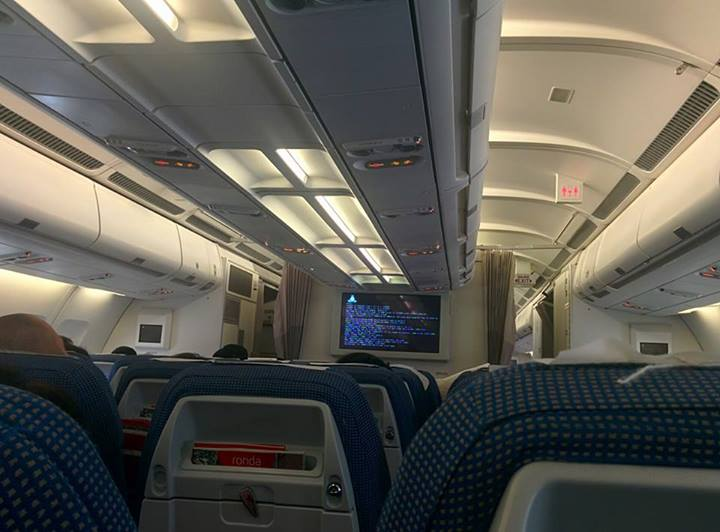
\includegraphics[width=0.7\linewidth]{Images/avion.jpg}
    \end{figure}
\end{frame}

\begin{frame}{Porque}
    \begin{itemize}
        \item Bajo/ningun coste
        \item Libertad
        \item Seguridad
        \item Orientado al usuario
        \item Hecho por y para desarrolladores
    \end{itemize}
\end{frame}

%%---------------------------
\section{Evolucion}
\begin{frame}{Microsoft}
    \pause
    \begin{figure}[tbph]
        \centering
        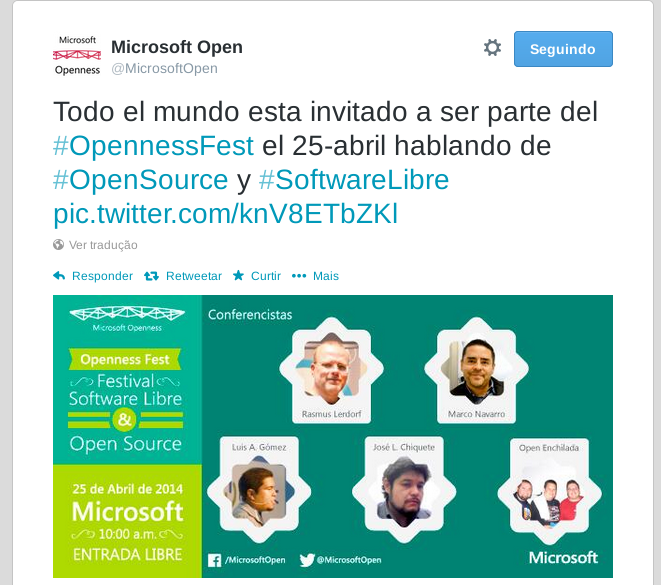
\includegraphics[width=0.8\linewidth]{Images/mof.png}
    \end{figure}
\end{frame}

\begin{frame}{Red Hat}
    \pause
    \begin{figure}[tbph]
        \centering
        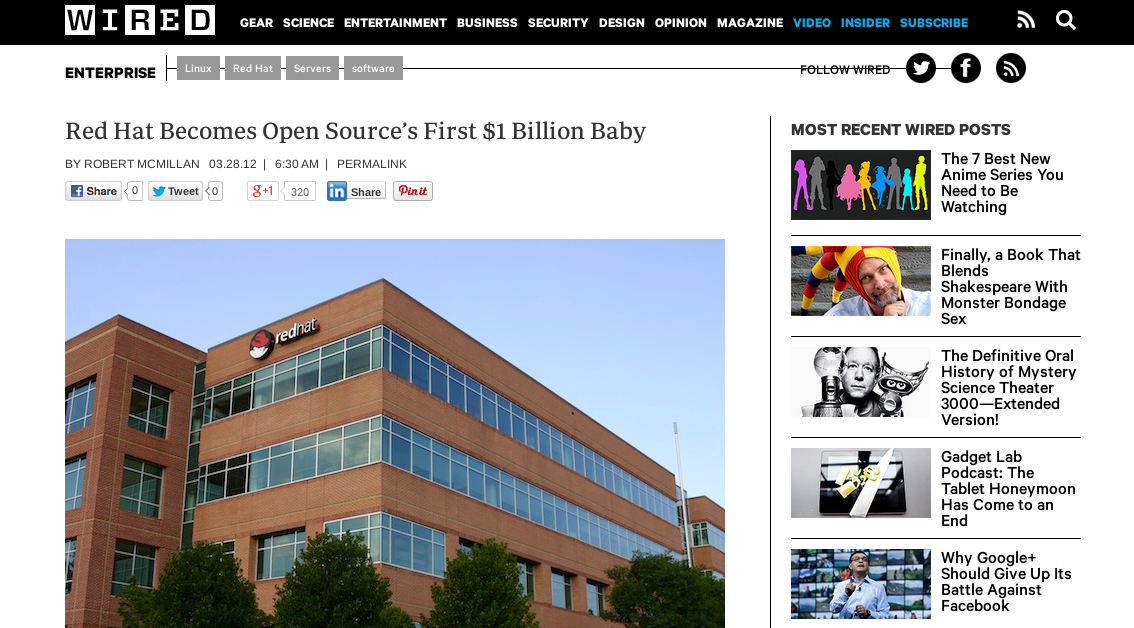
\includegraphics[width=0.8\linewidth]{Images/redhat.png}
    \end{figure}
\end{frame}

\begin{frame}{Super computers}
    \pause
    \begin{figure}[tbph]
        \centering
        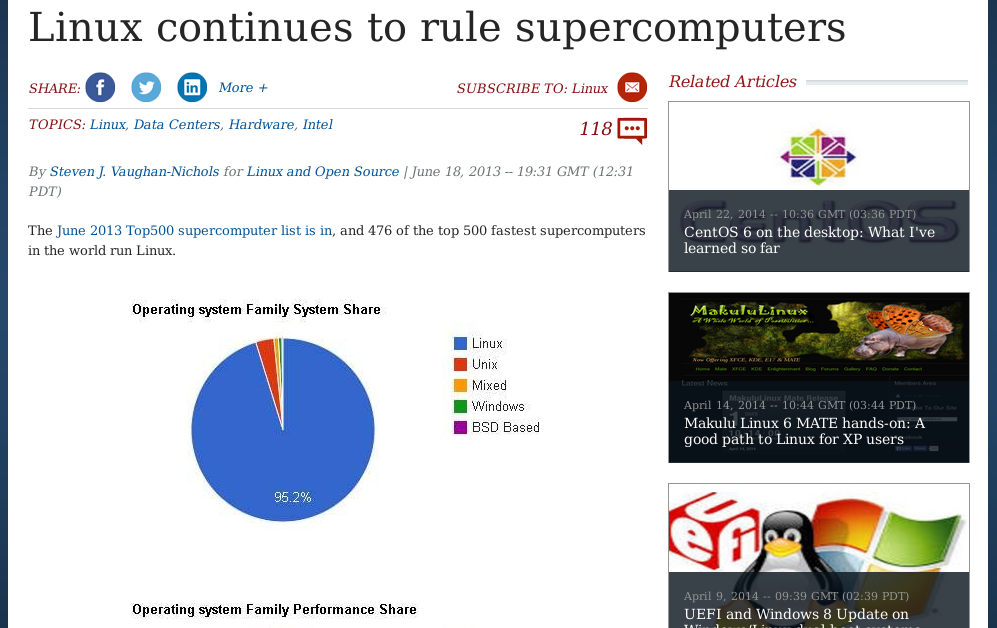
\includegraphics[width=0.8\linewidth]{Images/top500.png}
    \end{figure}
\end{frame}

\begin{frame}{Brasil}
    \pause
    \begin{figure}[tbph]
        \centering
        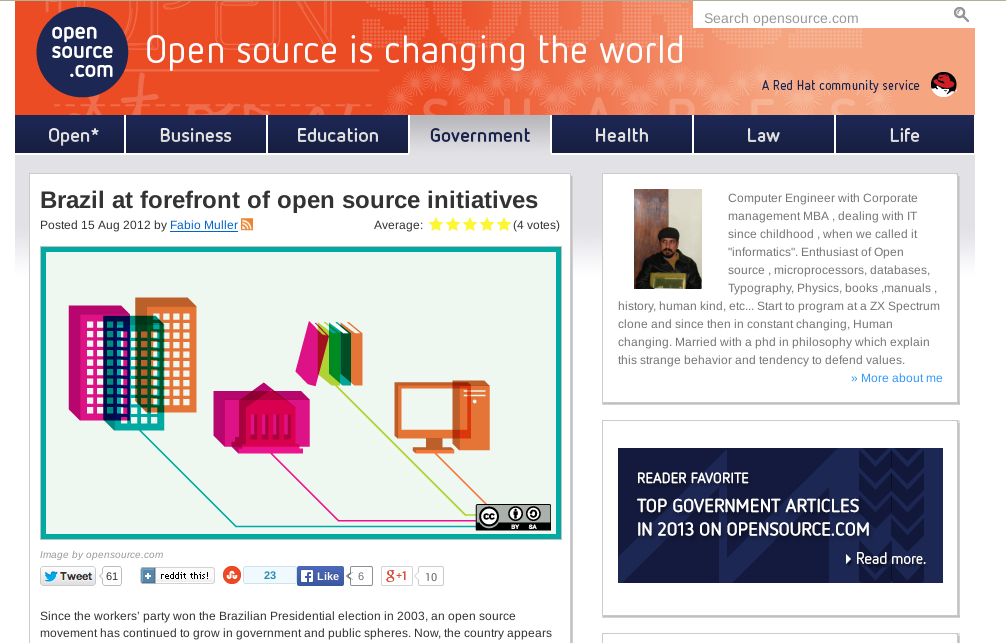
\includegraphics[width=0.8\linewidth]{Images/brazil.png}
    \end{figure}
\end{frame}


%%---------------------------
\section{Porque}

\begin{frame}{Egoismo racional}
La busqueda del propio interes es siempre racional
\end{frame}

\begin{frame}{}
1. Porque es divertido
\end{frame}

\begin{frame}{}
2. Porque abre muchas puertas
\end{frame}

\begin{frame}{}
3. Porque abre muchas puertas . . . laborales!
\end{frame}

\begin{frame}{}
4. Porque permite aprender
\end{frame}

\begin{frame}{}
6. Porque baja la barrera para iniciar su startup
\end{frame}

\begin{frame}{}
7. Porque es el presente y el futuro!
    \begin{figure}[tbph]
        \centering
        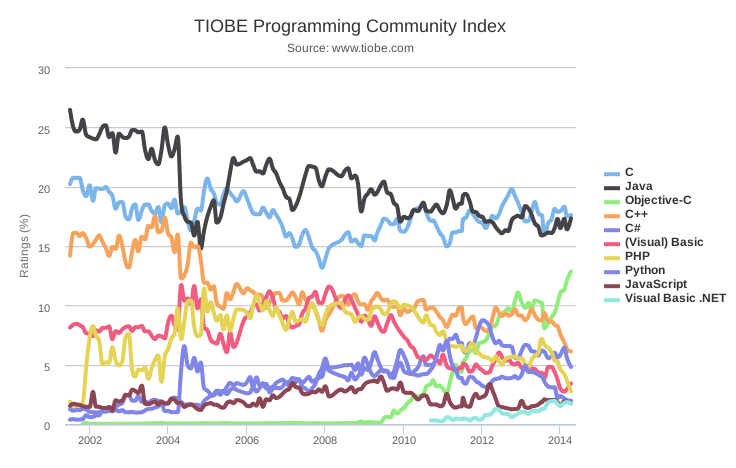
\includegraphics[width=0.7\linewidth]{Images/tiboe.png}
    \end{figure}
\end{frame}


\begin{frame}{¿Como inicio?}
    Ya lo hiciste
    \pause
    \begin{itemize}
    \item Grupos de usuarios
    \item Internet \& Google
    \item Listas de correo, foros, blogs, irc, etc.
    \item Empresas de soporte local
    \item Empresas de soporte internacional
    \end{itemize}
\end{frame}

\begin{frame}{¿Como inicio?}
\begin{itemize}
\item Xelalug (http://www.xelalug.org/)
\item Shekalug (http://www.shekalug.org/)
\item Ubuntu Guatemala, SLGT, GUUG, Guatejug.
\end{itemize}
\end{frame}

\section{Fin}

\begin{frame}{Gracias}
\begin{itemize}
\item tuxtor@shekalug.org
\item http://tuxtor.shekalug.org
\item http://github.com/tuxtor/slides
\end{itemize}
\begin{center}

\includegraphics[width=0.1\linewidth]{Images/cclogo}
\\
This work is licensed under a Creative Commons Attribution-ShareAlike 3.0 Guatemala License.
\end{center}
\end{frame}
\end{document}
